%  LaTeX support: latex@mdpi.com
%  For support, please attach all files needed for compiling as well as the log file, and specify your operating system, LaTeX version, and LaTeX editor.

%=================================================================
% pandoc conditionals added to preserve backwards compatibility with previous versions of rticles

\documentclass[nutrients,article,submit,moreauthors,pdftex]{Definitions/mdpi}


%% Some pieces required from the pandoc template
\setlist[itemize]{leftmargin=*,labelsep=5.8mm}
\setlist[enumerate]{leftmargin=*,labelsep=4.9mm}


%--------------------
% Class Options:
%--------------------

%---------
% article
%---------
% The default type of manuscript is "article", but can be replaced by:
% abstract, addendum, article, book, bookreview, briefreport, casereport, comment, commentary, communication, conferenceproceedings, correction, conferencereport, entry, expressionofconcern, extendedabstract, datadescriptor, editorial, essay, erratum, hypothesis, interestingimage, obituary, opinion, projectreport, reply, retraction, review, perspective, protocol, shortnote, studyprotocol, systematicreview, supfile, technicalnote, viewpoint, guidelines, registeredreport, tutorial
% supfile = supplementary materials

%----------
% submit
%----------
% The class option "submit" will be changed to "accept" by the Editorial Office when the paper is accepted. This will only make changes to the frontpage (e.g., the logo of the journal will get visible), the headings, and the copyright information. Also, line numbering will be removed. Journal info and pagination for accepted papers will also be assigned by the Editorial Office.

%------------------
% moreauthors
%------------------
% If there is only one author the class option oneauthor should be used. Otherwise use the class option moreauthors.

%---------
% pdftex
%---------
% The option pdftex is for use with pdfLaTeX. Remove "pdftex" for (1) compiling with LaTeX & dvi2pdf (if eps figures are used) or for (2) compiling with XeLaTeX.

%=================================================================
% MDPI internal commands - do not modify
\firstpage{1}
\makeatletter
\setcounter{page}{\@firstpage}
\makeatother
\pubvolume{1}
\issuenum{1}
\articlenumber{0}
\pubyear{2024}
\copyrightyear{2024}
%\externaleditor{Academic Editor: Firstname Lastname}
\datereceived{ }
\daterevised{ } % Comment out if no revised date
\dateaccepted{ }
\datepublished{ }
%\datecorrected{} % For corrected papers: "Corrected: XXX" date in the original paper.
%\dateretracted{} % For corrected papers: "Retracted: XXX" date in the original paper.
\hreflink{https://doi.org/} % If needed use \linebreak
%\doinum{}
%\pdfoutput=1 % Uncommented for upload to arXiv.org

%=================================================================
% Add packages and commands here. The following packages are loaded in our class file: fontenc, inputenc, calc, indentfirst, fancyhdr, graphicx, epstopdf, lastpage, ifthen, float, amsmath, amssymb, lineno, setspace, enumitem, mathpazo, booktabs, titlesec, etoolbox, tabto, xcolor, colortbl, soul, multirow, microtype, tikz, totcount, changepage, attrib, upgreek, array, tabularx, pbox, ragged2e, tocloft, marginnote, marginfix, enotez, amsthm, natbib, hyperref, cleveref, scrextend, url, geometry, newfloat, caption, draftwatermark, seqsplit
% cleveref: load \crefname definitions after \begin{document}

%=================================================================
% Please use the following mathematics environments: Theorem, Lemma, Corollary, Proposition, Characterization, Property, Problem, Example, ExamplesandDefinitions, Hypothesis, Remark, Definition, Notation, Assumption
%% For proofs, please use the proof environment (the amsthm package is loaded by the MDPI class).

%=================================================================
% Full title of the paper (Capitalized)
\Title{Substitution of red meat with legumes and risk of primary liver
cancer in 126,744 UK Biobank participants: a prospective cohort study}

% MDPI internal command: Title for citation in the left column
\TitleCitation{Substitution of red meat with legumes and risk of primary
liver cancer in 126,744 UK Biobank participants: a prospective cohort
study}

% Author Orchid ID: enter ID or remove command
%\newcommand{\orcidauthorA}{0000-0000-0000-000X} % Add \orcidA{} behind the author's name
%\newcommand{\orcidauthorB}{0000-0000-0000-000X} % Add \orcidB{} behind the author's name


% Authors, for the paper (add full first names)
\Author{Niels Bock$^{1}$\href{https://orcid.org/0009-0005-7373-1589}
{\orcidicon}, Fie
Langmann$^{1}$\href{https://orcid.org/0000-0003-3474-9346}
{\orcidicon}, Luke W. Johnston$^{1,
2}$\href{https://orcid.org/0000-0003-4169-2616}
{\orcidicon}, Daniel B. Ibsen$^{1, 2, 3,
4}$\href{https://orcid.org/0000-0002-7038-4770}
{\orcidicon}, Christina C. Dahm$^{1,
*}$\href{https://orcid.org/0000-0003-0481-2893}
{\orcidicon}}


%\longauthorlist{yes}


% MDPI internal command: Authors, for metadata in PDF
\AuthorNames{Niels Bock, Fie Langmann, Luke W. Johnston, Daniel B.
Ibsen, Christina C. Dahm}

% MDPI internal command: Authors, for citation in the left column
%\AuthorCitation{Lastname, F.; Lastname, F.; Lastname, F.}
% If this is a Chicago style journal: Lastname, Firstname, Firstname Lastname, and Firstname Lastname.
\AuthorCitation{Bock, N.; Langmann, F; Johnston, LW; Ibsen, DB; Dahm,
CC.}

% Affiliations / Addresses (Add [1] after \address if there is only one affiliation.)
\address{%
$^{1}$ \quad Department of Public Health, Aarhus University, Aarhus,
Denmark; \\
$^{2}$ \quad Steno Diabetes Center Aarhus, Aarhus University Hospital,
Aarhus N, Denmark; \\
$^{3}$ \quad Department of Nutrition, Exercise and Sports, University of
Copenhagen, Copenhagen, Denmark; \\
$^{4}$ \quad MRC Epidemiology Unit, School of Clinical Medicine,
University of Cambridge, Cambridge, United Kingdom; \\
}

% Contact information of the corresponding author
\corres{Correspondence: \href{mailto:CCD@ph.au.dk}{\nolinkurl{CCD@ph.au.dk}}.}

% Current address and/or shared authorship








% The commands \thirdnote{} till \eighthnote{} are available for further notes

% Simple summary

%\conference{} % An extended version of a conference paper

% Abstract (Do not insert blank lines, i.e. \\)
\abstract{Purpose: Primary liver cancer is on the rise worldwide,
partially due to poor diets and sedentary lifestyles. Shifting to more
plant-based diets may lower the risk. We aimed to estimate the effect of
replacing unprocessed red meat, processed red meat and total red meat
with legumes on primary liver cancer in a free-living population.
Methods: We analyzed data from 126,744 UK Biobank participants who
completed \(\geq\) 2 24-hour diet recalls. Baseline characteristics were
collected from the initial assessment visit. Information on liver cancer
diagnoses was collected via external linkage to inpatient hospital
episodes or central cancer registries. Cox proportional hazards
regression models were used to estimate substitution of 15 g/day of
legumes with 15 g/day of total red meat, unprocessed red meat and
processed red meat on liver cancer risk, using the leave-one-out food
substitution model. Results: During a median follow-up time of 11.3
years, 173 participants developed liver cancer. In the fully adjusted
models, no association was observed when substituting 15 g/day of
legumes with total red meat (HR: 0.98 (95\% CI 0.93-1.04)), unprocessed
red meat (HR: 0.97 (95\% CI 0.91-1.03)) or processed red meat (HR: 1.02
(95\% CI 0.93-1.13)). Conclusion: Overall, little evidence of an
association between replacing red meat with legumes and liver cancer was
observed. Further research in larger study populations with longer
follow-up time is warranted.}


% Keywords
\keyword{Food Substitutions; liver cancer; red meat; legumes.}

% The fields PACS, MSC, and JEL may be left empty or commented out if not applicable
%\PACS{J0101}
%\MSC{}
%\JEL{}

%%%%%%%%%%%%%%%%%%%%%%%%%%%%%%%%%%%%%%%%%%
% Only for the journal Diversity
%\LSID{\url{http://}}

%%%%%%%%%%%%%%%%%%%%%%%%%%%%%%%%%%%%%%%%%%
% Only for the journal Applied Sciences

%%%%%%%%%%%%%%%%%%%%%%%%%%%%%%%%%%%%%%%%%%

%%%%%%%%%%%%%%%%%%%%%%%%%%%%%%%%%%%%%%%%%%
% Only for the journal Data



%%%%%%%%%%%%%%%%%%%%%%%%%%%%%%%%%%%%%%%%%%
% Only for the journal Toxins


%%%%%%%%%%%%%%%%%%%%%%%%%%%%%%%%%%%%%%%%%%
% Only for the journal Encyclopedia


%%%%%%%%%%%%%%%%%%%%%%%%%%%%%%%%%%%%%%%%%%
% Only for the journal Advances in Respiratory Medicine
%\addhighlights{yes}
%\renewcommand{\addhighlights}{%

%\noindent This is an obligatory section in “Advances in Respiratory Medicine”, whose goal is to increase the discoverability and readability of the article via search engines and other scholars. Highlights should not be a copy of the abstract, but a simple text allowing the reader to quickly and simplified find out what the article is about and what can be cited from it. Each of these parts should be devoted up to 2~bullet points.\vspace{3pt}\\
%\textbf{What are the main findings?}
% \begin{itemize}[labelsep=2.5mm,topsep=-3pt]
% \item First bullet.
% \item Second bullet.
% \end{itemize}\vspace{3pt}
%\textbf{What is the implication of the main finding?}
% \begin{itemize}[labelsep=2.5mm,topsep=-3pt]
% \item First bullet.
% \item Second bullet.
% \end{itemize}
%}


%%%%%%%%%%%%%%%%%%%%%%%%%%%%%%%%%%%%%%%%%%


% tightlist command for lists without linebreak
\providecommand{\tightlist}{%
  \setlength{\itemsep}{0pt}\setlength{\parskip}{0pt}}



\usepackage{longtable}
\usepackage{booktabs}
\usepackage{caption}
\usepackage{colortbl}
\usepackage{array}
\usepackage{anyfontsize}

\begin{document}



%%%%%%%%%%%%%%%%%%%%%%%%%%%%%%%%%%%%%%%%%%

This research has been conducted using the UK Biobank Resource under
Application Number 81520.

\hypertarget{sec1}{%
\section{Background}\label{sec1}}

Hepatocellular carcinoma (HCC) is the sixth most common cancer in the
world and the third leading cause of cancer-related death with viral
hepatitis being the leading risk factor \citep{Massarweh2017}. In
low-infection populations, modifiable risk factors, such as dietary
habits, may play an increasing role in HCC pathogenesis as non-alcoholic
fatty liver disease (NAFLD) has become the leading cause of liver
cirrhosis \citep{Younossi2016, Younossi2020} that may in turn progress
to HCC. A western dietary pattern high in fats and red meats and
concurrently low in fruits, vegetables, and whole grains has been
associated with NAFLD progression \citep{Guo2022}. The prevalence of
NAFLD-related HCC cases is an increasing global problem
\citep{Younossi2016}. It is estimated that the prevalence of
NAFLD-related HCC in the US will increase by 146\%, while incident
NAFLD-related HCC cases will increase by 137\% by 2030
\citep{Estes2018}.

The second most common primary liver cancer is the intrahepatic
cholangiocarcinoma (ICC) \citep{Khan2019}. While HCC emerges from the
liver parenchyma, ICC emerges from the bile duct. Despite being a
relatively rare cancer, ICC is characterized by its aggressiveness, late
diagnosis and poor survival \citep{kirstein2016}. It is estimated that
the incidence of ICC is increasing in populations that are not burdened
by known infectous and environmental risk factors \citep{Bergquist2015}.
Recent meta-analyses of observational studies and clinical trials have
shown a significant adverse association between NAFLD and ICC
\citep{Wongjarupong2017, corrao2020}.

The impact of specific food groups on liver cancer risk is not well
known. Observational studies suggest that intake of coffee, vegetables
and whole grains may lower HCC risk
\citep{zhang2013, yang2014, Liu2021, Bhurwal2020}. The protective
properties of these foods are proposedly due to their content of dietary
fibers and polyphenols, which are also defining components of legumes.
The health benefits of legumes extend to improved glycemic control and
hypotensive and anticarcinogenic properties with observed inverse
associations with cardiovascular disease and colorectal cancer
\citep{viguiliouk2019, jin2022}. Two large prospective cohort studies
found evidence of inverse associations between legume consumption and
risk of HCC \citep{zhang2013, Liu2021}. However, replacement foods were
not specified in these studies, which fails to reflect that an increase
in intake of one food is at the expense of a concomitantly decreased
intake of another food. Studies on substituting plant-based proteins for
animal-based proteins are important if we are to lower the climate
impacts of our diets \citep{RN71}. Although previous research has
investigated substitution of animal-based proteins with plant-based
proteins in relations to NAFLD \citep{Zhang2023}, research on
substituting meats with legumes in relation to risk of HCC and ICC is
sparse. This leaves a substantial gap in the current knowledge on the
beneficial effects on primary liver cancer from substituting red meat
with legumes.

The low incidence of liver cancer in populations not burdened by viral
hepatitis complicates observational prospective research designs;
nonetheless, the prospects of the burden of liver cancer on public
health warrant investigation of preventative measures. Thus, the main
aim of this study was to estimate the association between replacing
unprocessed red meat, processed red meat and total red meat with legumes
on primary liver cancer in a free-living population.

\hypertarget{sec2}{%
\section{Research Design and Methods}\label{sec2}}

\hypertarget{subsec1}{%
\subsection{Study population}\label{subsec1}}

The UK Biobank, a population-based prospective cohort, was initiated in
2006. \citep{sudlow2015} During 2006-2010, more than 500,000
participants, aged 40-69, were recruited and visited designated
assessment centres across the UK. Participants provided information
about age, sex, sociodemographic factors (education, Townsend
deprivation index, living alone) and lifestyle factors (smoking, alcohol
consumption, physical activity) via touch screen questionnaires and
computer-assisted interviews. Anthropometric data (waist circumference)
were collected via physical measurements \citep{RN113}.

\hypertarget{subsec2}{%
\subsection{Dietary assessment}\label{subsec2}}

A web-based 24-hour dietary recall was administered at the end of the
initial assessment visit for the last 70,000 recruited participants
\citep{RN115}. From February 2011 to April 2012, 320,000 participants
who had provided an e-mail address were invited on four separate
occasions to complete the 24-hour dietary recall, the Oxford WebQ, of
which 210,947 participants completed at least one. The Oxford WebQ
covered 206 food items and 32 beverage items commonly consumed in the
UK. Intakes were reported in standard units of measurements, e.g.,
servings, cups, slices, etc. with intake categories ranging from 0 to 3+
units \citep{piernas2021}. The Oxford WebQ has been validated against
interviewer-based 24-hour dietary recalls and biomarkers
\citep{Liu2011, Greenwood2019}.

Researchers defined 79 food groups and 14 beverage groups from the
Oxford WebQ using the UK National Diet and Nutrition Survey categories
\citep{piernas2021}. These food and beverage groups were used when
defining the food groups used in the substitution analyses (Table
\ref{tab-food-group}). Legumes were defined as dietary pulses, baked
beans, tofu-based products, peas, hummus, soy drinks, and soy-based
desserts and yogurt. Red meat intake was defined as intake of beef,
pork, lamb, or other meat, including offal. Processed red meat intake
was defined as sausages, bacon (with and without fat), ham, or liver
pate. Other food groups included were animal-based foods, unhealthy
plant-based foods, healthy plant-based foods, and alcoholic beverages
(Table \ref{tab-food-group}). Animal-based and healthy and unhealthy
plant-based food foods were grouped based on plant-based diet indices
from previous studies
\citep{Thompson2023, Heianza2021, Satija2017, Satija2016}.

As a single 24-hour dietary recall does not assess habitual dietary
intake and variation in diet over time at an individual level
\citep{thompson2013, gurinovic2017}, only participants who completed two
or more Oxford WebQs were eligible for inclusion in this study.

\hypertarget{subsec3}{%
\subsection{Liver cancer assessment}\label{subsec3}}

Liver cancer was defined according to ICD-10 diagnosis codes C22.0 for
Hepatocellular carcinoma (HCC) or C22.1 for Intrahepatic
cholangiocarcinoma (ICC) and ICD-9 diagnosis codes 1550 Malignant
neoplasm of liver, primary or 1551 Malignant neoplasm of intrahepatic
bile ducts. Incident and prevalent cases of liver cancer and
corresponding diagnosis dates were obtained via external linkage to
central cancer registries or hospital inpatient episodes
\citep{RN112, RN114}.

\hypertarget{subsec4}{%
\subsection{Assessment of confounders}\label{subsec4}}

Confounders were defined \emph{a priori} from a review of the background
literature and illustrated using directed acyclic graphs (Figure
\ref{fig:fig2}). The following confounding variables were selected: age
at baseline (years, continuous), sex (male, female), educational level
(high: College or University degree, intermediate: A levels/AS levels, O
levels/GCSEs, or equivalent, low: none of the previous mentioned),
Townsend Deprivation Index (continuous), Living alone (yes, no), waist
circumference (cm, continuous), physical activity (above/below the 2017
UK Physical activity guidelines of 150 minutes of moderate activity per
week or 75 minutes of vigorous activity, or unknown), smoking (pack
years as a proportion of lifespan exposed to smoking, continous), and
alcohol intake (g/day, continuous). All confounders except age were
selected from the initial assessment visit before the start of
follow-up.

\hypertarget{subsec5}{%
\subsection{The substitution model}\label{subsec5}}

The substitution analyses were conducted by by modelling replacement of
an equal mass of meat with legumes. The portion size of the substitution
was set to 15 g of legumes for 15 g of red meat to ensure that
substitutions were below the mean intake of any of the substituted food
groups in the cohort. The substitutions were modeled using the
leave-one-out-approach in which variables for every food group along
with a variable for total food intake are included, except the food
group that are to be substituted \citep{Ibsen2021}. To estimate
substitution of 15 g of all red meats (red and processed) with 15 g of
legumes, the following model was defined:

\begin{align}
\log(h(t;x)) &= \log(h_0(t)) + \beta_1 \text{Legumes (15g)} \hspace{0.5em} + \nonumber \\
&\quad \hspace{0.5em} \beta_2 \text{Total food intake (g)} + \beta_3 \text{Other food groups (g)} + \beta_4 \text{Covariates}
\end{align}

\noindent When substituting only unprocessed red meat with legumes,
processed red meat was added to the model:

\begin{align}
\log(h(t;x)) &= \log(h_0(t)) + \beta_1 \text{Legumes (15g)} + \beta_2 \text{Processed red meat (15g)} \hspace{0.5em} + \nonumber \\
&\quad \hspace{0.5em} \beta_3 \text{Total food intake (g)} + \beta_4 \text{Other food groups (g)} + \beta_5 \text{Covariates}
\end{align}

\noindent When substituting only processed red meat with legumes, red
meat was added to the model:

\begin{align}
\log(h(t;x)) &= \log(h_0(t)) + \beta_1 \text{Legumes (15g)} + \beta_2 \text{Unprocessed red meat (15g)} \hspace{0.5em} + \nonumber \\
&\quad \hspace{0.5em} \beta_3 \text{Total food intake (g)}  + \beta_4 \text{Other food groups (g)} + \beta_5 \text{Covariates}
\end{align}

\noindent The performance of the leave-one-out model when modeling equal
mass substitutions has been validated against simulated data
\citep{Tomova2022}.

\hypertarget{subsec6}{%
\subsection{Statistical analysis}\label{subsec6}}

Multivariable-adjusted Cox proportional hazards regression models were
used to estimate hazard ratios (HR) with corresponding 95\% confidence
intervals (CI) with age as the underlying timescale. Participants were
followed from the date of their last completed Oxford WebQ until the
occurrence of the event of interest or due to right censoring, whichever
came first. Participants were right censored in the event of death, loss
to follow-up, or administrative end of follow-up (October 31, 2022). Two
levels of adjustments were added to the substitution model. Model 1 was
minimally adjusted for age (as the underlying timescale), total weight
of food and beverage intake, and all other food groups to fit the
substitution model. Model 2 was further adjusted for sex, educational
level, Townsend Deprivation Index, living alone, physical activity,
smoking, alcohol intake, and waist circumference.

In secondary analyses, each cancer type was analysed separately to
evaluate if the pooling of HCC and ICC as one outcome in the main
analysis was justified. Furthermore, to estimate the association of
legume intake with liver cancer regardless of other dietary components,
legume consumers (divided into quartiles) were compared to
non-consumers.

To evaluate the robustness of the main analyses, sensitivity analyses
were performed on subsamples of participants by excluding those with
high alcohol intake (exclusion of the upper decile of alcohol intake
(g/day) by sex), implausible energy intake (exclusion of participants
below the 2.5th percentile and above the 97.5th percentile of energy
intake (kJ/day) by sex), any liver disease before baseline, any type of
cancer before baseline, and fewer than 3 completed Oxford WebQs. As
neither the central cancer registries nor the hospital inpatient
registries were complete, liver cancer diagnoses retrieved from death
registries, which were more up-to-date, were included in a sensitivity
analysis to test for outcome misclassification. Lastly, one of our
causal assumptions was that anthropometry confounded the causal
relationship between replacing red meat with legumes and liver cancer;
however, strong arguments exist giving support to anthropometry being a
mediator between diet and health outcomes. Thus, to test for erroneously
conditioning on a potential mediator, waist circumference was removed in
a sensitivity analysis. Sensitivity analyses were modeled as the fully
adjusted models in the main analyses.

All analyses were conducted in R (version 4.1.1) with a significance
level of 5 \%.

\hypertarget{sec3}{%
\section{Results}\label{sec3}}

After excluding participants with liver cancer before baseline,
participants lost to follow-up before baseline, and participants with
errors in dietary data, 126,744 participants who had completed two or
more Oxford WebQs remained (Figure \ref{fig:fig1}).

\begin{figure*}

{\centering 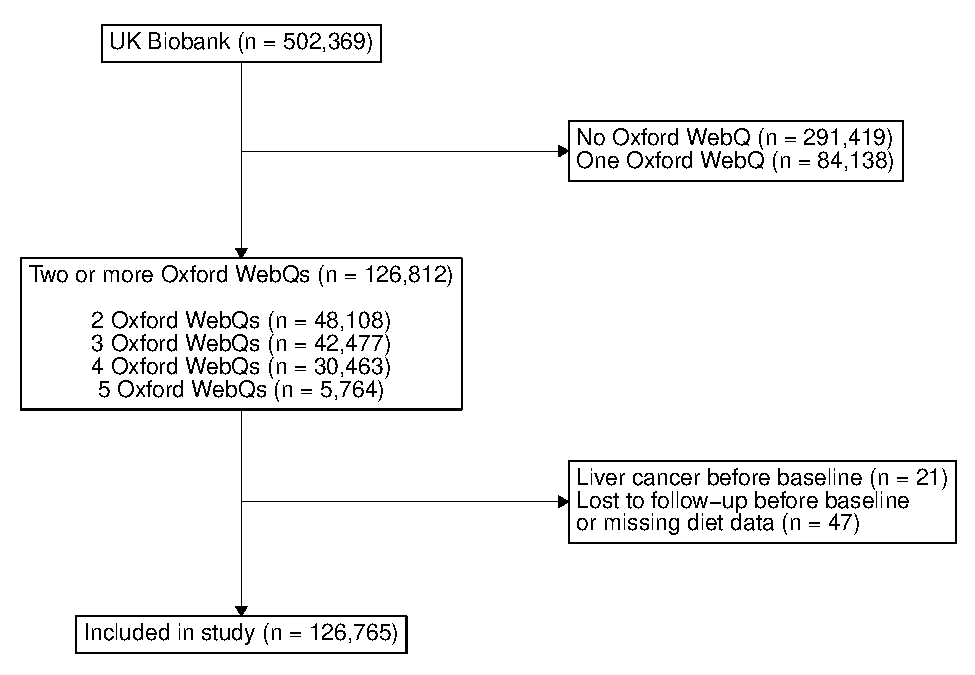
\includegraphics[width=1\linewidth,]{legliv-nutrients_files/figure-latex/fig1-1} 

}

\caption{Flowchart of included participants. Missing diet data were merged with loss to follow-up before baseline due to n being less than 5. It should be noted that not all UK Biobank participants were invited to complete an Oxfords WebQ. Only the last 70,000 participants to visit an assessment center were asked to complete an Oxford WebQ at the end of their visit. Further Oxford WebQs were sent to ~320,000 participants who provied an e-mail adress.}\label{fig:fig1}
\end{figure*}

During a median follow-up time of 11.3 years, 173 participants developed
liver cancer. Participants who developed liver cancer were older at
baseline, were more likely to be male, have a higher waist
circumference, be less physically active, and fewer had never smoked,
compared to all included participants (Table \ref{tab1}).

\begin{table}[t]
\caption{
{\small \textbf{Baseline characteristics of UK Biobank participants who completed \(\geq\) 2 Oxford WebQ 24-hour diet recall.}}
}\label{tab1} 
\fontsize{9.0pt}{10.8pt}\selectfont
\begin{tabular*}{1\linewidth}{@{\extracolsep{\fill}}lcc}
\toprule
 & \textbf{Cohort} & \textbf{Liver cancer} \\ 
\cmidrule(lr){2-2} \cmidrule(lr){3-3}
\textbf{Variable} & \textbf{N = 126,744}\textsuperscript{\textit{1}} & \textbf{N = 173}\textsuperscript{\textit{1}} \\ 
\midrule\addlinespace[2.5pt]
{\bfseries Typical diet yesterday}\textsuperscript{\textit{2}} & 73,213 (58\%) & 105 (61\%) \\ 
{\bfseries Age, years} & 60 (53, 65) & 64.0 (60.0, 68.0) \\ 
{\bfseries Sex} &  &  \\ 
    Female & 70,659 (56\%) & 65 (38\%) \\ 
    Male & 56,085 (44\%) & 108 (62\%) \\ 
{\bfseries Educational level}\textsuperscript{\textit{3}} &  &  \\ 
    High & 59,416 (47\%) & 76 (44\%) \\ 
    Intermediate & 41,817 (33\%) & 52 (30\%) \\ 
    Low & 25,472 (20\%) & 45 (26\%) \\ 
    Missing & 39 &  \\ 
{\bfseries Townsend Deprivation Index} & -2.4 (-3.8, 0.0) & -2.6 (-3.7, -0.7) \\ 
    Missing & 149 &  \\ 
{\bfseries Living alone} & 22,658 (18\%) & 34 (20\%) \\ 
    Missing & 171 &  \\ 
{\bfseries Physical activity}\textsuperscript{\textit{4}} &  &  \\ 
    Above & 58,111 (46\%) & 61 (35\%) \\ 
    Below & 50,712 (40\%) & 79 (46\%) \\ 
    Missing & 17,921 (14\%) & 33 (19\%) \\ 
{\bfseries Smoking} &  &  \\ 
    Never & 72,583 (57\%) & 75 (43\%) \\ 
    Ever & 54,122 (43\%) & 98 (57\%) \\ 
    Missing & 39 &  \\ 
{\bfseries Alcohol intake, g/day} & 11 (0, 26) & 11 (0, 29) \\ 
{\bfseries Waist circumference, cm} & 88 (79, 97) & 98 (89, 107) \\ 
    Missing & 168 &  \\ 
\bottomrule
\end{tabular*}
\begin{minipage}{\linewidth}
\textsuperscript{\textit{1}}Median (IQR) for continous variables; n (\%) for categorical variables\\
\textsuperscript{\textit{2}}Participants who reported eating a typical diet yesterday for all completed diet questionnaires.\\
\textsuperscript{\textit{3}}High: College or University degree;
Intermediate: A levels/AS levels, O levels/GCSEs, or equivalent;
Low: none of the previous mentioned.\\
\textsuperscript{\textit{4}}Above or below the 2017 UK Physical activity guidelines of 150 minutes of moderate activity per week or 75 minutes of vigorous activity.\\
\end{minipage}
\end{table}

Mean daily energy and total food intakes as well as daily intake of all
specified food groups in grams are presented in Table \ref{tabdiet}.

\begin{table}[t]
\caption{
{\small \textbf{Daily dietary intake of food groups, total food and total energy intake in UK Biobank participants who completed \(\geq\) 2 Oxford WebQ 24-hour diet recall.}}
}\label{tabdiet} 
\fontsize{9.0pt}{10.8pt}\selectfont
\begin{tabular*}{1\linewidth}{@{\extracolsep{\fill}}lcc}
\toprule
 & \textbf{Cohort} & \textbf{Liver cancer} \\ 
\cmidrule(lr){2-2} \cmidrule(lr){3-3}
\textbf{Daily food intake} & \textbf{N = 126,744}\textsuperscript{\textit{1}} & \textbf{N = 173}\textsuperscript{\textit{1}} \\ 
\midrule\addlinespace[2.5pt]
\multicolumn{3}{l}{{\bfseries Total food intake}} \\ 
\midrule\addlinespace[2.5pt]
Energy, kJ & 8,430 (7,179, 9,856) & 8,579 (7,413, 10,048) \\ 
Weight, g & 3,144 (2,720, 3,621) & 3,162 (2,737, 3,659) \\ 
\midrule\addlinespace[2.5pt]
\multicolumn{3}{l}{{\bfseries Food groups, g/day}} \\ 
\midrule\addlinespace[2.5pt]
Legumes & 11 (0, 34) & 8 (0, 35) \\ 
Red and processed meat & 53 (15, 86) & 60 (30, 95) \\ 
Red meat & 30 (0, 60) & 45 (0, 73) \\ 
Processed meat & 9 (0, 30) & 8 (0, 31) \\ 
Other animal-based foods\textsuperscript{\textit{2}} & 475 (361, 603) & 448 (322, 604) \\ 
Healthy plant-based foods\textsuperscript{\textit{3}} & 1,806 (1,454, 2,198) & 1,791 (1,365, 2,158) \\ 
Unhealthy plant-based foods\textsuperscript{\textit{4}} & 472 (324, 662) & 491 (365, 698) \\ 
Alcoholic beverages & 132 (0, 342) & 144 (0, 375) \\ 
\bottomrule
\end{tabular*}
\begin{minipage}{\linewidth}
\textsuperscript{\textit{1}}Median (IQR)\\
\textsuperscript{\textit{2}}Other animal-based foods include: poultry, fish, dairy, eggs, and mixed dishes with animal products.\\
\textsuperscript{\textit{3}}Healthy plant-based foods include: whole grains, vegetables, fruits, nuts, plant oils, and beverages (coffee, tea, water).\\
\textsuperscript{\textit{4}}Unhealthy plant-based foods includes: refined grains, potatoes, mixed vegetarian dishes, sweets and snacks, fruit juice, and sugar sweetened beverages.\\
\end{minipage}
\end{table}

No evidence of associations was found for substituting 15 g/day of
legumes with 15 g/day of total red meat, unprocessed red meat, or
processed red meat and risk of primary liver cancer in Model 1 (Table
\ref{tab-main}: total red meat: HR: 0.98, 95\% CI: 0.93-1.04;
unprocessed red meat: HR: 0.97, 95\% CI: 0.91-1.03; processed red meat:
HR: 1.02, 95\% CI: 0.93-1.13). The estimated associations changed
minimally with further adjustments. There was weak evidence of an
association between replacement of processed red meat with legumes ( HR:
1.09, 95\% CI: 0.98-1.20; Table \ref{tab-main}).

\begin{table}[t]
\caption{
{\small \textbf{Substitution of total meat, red meat and processed meat with legumes and hazard ratios and 95\% confidence intervals for primary liver cancer.}}
}\label{tabmain} 
\fontsize{9.0pt}{10.8pt}\selectfont
\begin{tabular*}{1\linewidth}{@{\extracolsep{\fill}}lcc}
\toprule
 & {\bfseries \textbf{Model 1}}\textsuperscript{\textit{1}} & {\bfseries \textbf{Model 2}}\textsuperscript{\textit{2}} \\ 
\cmidrule(lr){2-2} \cmidrule(lr){3-3}
\textbf{15 g/day of legumes replacing:} & \textbf{HR} \textbf{(95\% CI)} & \textbf{HR} \textbf{(95\% CI)} \\ 
\midrule\addlinespace[2.5pt]
Total red meat & 0.98 (0.93-1.04) & 1.02 (0.96-1.08) \\ 
Unprocessed red meat & 0.97 (0.91-1.03) & 1.00 (0.94-1.07) \\ 
Processed red meat & 1.02 (0.93-1.13) & 1.09 (0.98-1.20) \\ 
\bottomrule
\end{tabular*}
\begin{minipage}{\linewidth}
\textsuperscript{\textit{1}}Adjusted for age (as underlying timescale), other food groups, and total food intake.\\
\textsuperscript{\textit{2}}Further adjusted for sex, educational level, Townsend deprivation index, living alone, physical activity, smoking, alcohol intake, and waist circumference.\\
\end{minipage}
\end{table}

In secondary analyses, when analyzing the associations between
replacement of red meat with legumes and HCC or ICC separately, weak
evidence of a higher risk of HCC was observed (Table \ref{tab-cancer},
total red meat: HR: 1.06, 95\% CI: 0.97-1.16; unprocessed red meat: HR:
1.05, 95\% CI: 0.96-1.15; processed red meat: HR: 1.09, 95\% CI:
0.95-1.26). This was opposite for replacement of total red meat and
unprocessed red meat and ICC (total red meat: HR: 0.97, 95\% CI:
0.90-1.05; unprocessed red meat: HR: 0.95, 95\% CI: 0.87-1.03) but not
for processed red meat ( HR: 1.07, 95\% CI: 0.93- 1.22, Table
\ref{tab-cancer}). The magnitude or direction of associations were not
significantly different across strata of liver cancer types.

In the adjusted non-substitution analysis, only the first quartile of
legume intake (mean intake 6.3 grams/day) was associated with a lower
risk of liver cancer, compared to no intake (HR: 0.59, 95\% CI:
0.35-0.98); no associations were observed for quartiles 2, 3 or 4
compared to no intake (Table \ref{tab-legume}).

In sensitivity analyses, excluding participants based on high alcohol
intake, implausible energy intake, any liver disease or cancer before
baseline, or fewer than 3 completed Oxford WebQs did not alter the
estimates appreciably. Similar results were also found when including
death registries as a source of liver cancer cases and when excluding
waist circumference from the fully adjusted analysis (Table
\ref{tab-sens}).

\hypertarget{sec4}{%
\section{Discussion}\label{sec4}}

Contrary to our hypothesis, this study we showed little evidence of an
association between replacing 15 g/day of red or processed meat with
legumes on risk of primary liver cancer. The estimates were robust to
sensitivity analyses. When investigating liver cancer types separately,
replacing total red meat and unprocessed red meat with legumes showed
some weak evidence of an inverse association with ICC. The results for
legume intake without specified substitutions did not show a clear
pattern of association.

The prospective longitudinal design of this study established
temporality between the diet exposure and liver cancer outcome, and the
large sample size enabled analyses of a rare cancer. Further, our
specified substitution analyses have some strengths in contrast to
traditional methods in nutritional epidemiology through examining the
effect of consuming a food or nutrient while holding all other foods
constant. The substitution is easily interpretable and reflects the
implications that an increased intake of a food is at the expense a
decreased intake of other foods. In that sense, the food substitution
model mimics some aspects of a randomized controlled design. A
limitation of this research design was that the low intake of the
substituted foods in this population restricted the size of the
substitution, which may in turn have restricted findings of clinically
significant effect sizes.

Information on dietary intake was collected using self-reported 24-hour
diet recall questionnaires, which may have introduced measurement error
partly due 24-hour recalls not reflecting past dietary intake. However,
estimates were robust to exclusion of participants with fewer than three
completed Oxford WebQs, indicating that at least two 24-hour diet recall
measurements were sufficient to account for natural flucturations in
dietary intake over time. A validation study of the Oxford WebQ found
some person-specific biases within participants with a higher BMI having
greater disparities for correlation with true intakes for some nutrients
\citep{Greenwood2019}. We did not adjust for BMI; however, adjusting for
waist circumference did not change our estimates significantly, lending
some support to sufficient adjustment of person specific bias. Finally,
by specifying that the dietary exposure was collected on at least two
occasions, our study population suffered considerable attrition. This is
unlikely to be completely at random, and most likely resulted in a study
population with greater focus on their dietary habits. For example, the
mean intake of processed meat was low in our study population. If a diet
consisting of higher intakes of healthier plant-based foods is
associated with lower liver cancer incidence, our study population may
be at lower risk overall, thus reducing the power of our study to detect
an association.

None of the registries used to determine a diagnosis of liver cancer
were complete or up-to-date at the time of analysis \citep{RN112}. Data
from external providers, such as the NHS England, NHS Central Register
or National Records of Scotland, were estimated to be mostly complete by
the UK Biobank at various dates, ranging from 31 December 2016 for
cancer data from Wales to 31 October 2022 for hospital inpatient data
from England \citep{RN114}. This could introduce misclassification of
the outcome, as individuals with liver cancer may not be identified as
cases. However, the estimates were robust in a sensitivity analysis that
included death registries as an additional source of liver cancer
diagnoses to accommodate missing outcome events. Incorrectly classifying
non-cases as cases would lead to attenuation of our results, but this is
unlikely due to register linkage. Though health registries may have been
only partially up to date, using registries almost eliminates selection
bias due to loss to follow-up.

The relatively low number of events limited our ability to adjust for
confounding factors. Excessive adjustment parameters per event can
compromise the validity of the multivariable Cox regression model,
potentially causing biased estimates. To ensure statistical validity, we
aimed for at least 10 events per variable in the main analysis by
limiting the number of adjustment levels, using fewer and broader food
groups, and fewer levels for categorical covariates. This approach was
guided by our \emph{a priori} causal assumptions. Although this method
helped maintain statistical validity, it may have increased residual
confounding by diluting the importance of specific food groups.
Additionally, risk factors that we could not adjust for, such as
aflatoxin B1, a known liver carcinogen, may have contributed to residual
confounding.

Contrary to our hypothesis, replacing processed red meat with legumes
was associated with a non-significant increase in risk of primary liver
cancer, with a greater effect size compared to unprocessed red meat.
This pattern persisted across all sensitivity analyses. However, the
estimates for processed red meat were labeled with less confidence,
partly due to the low median intake. The findings of this current study
align with other research in the UK Biobank, where unprocessed red meat
intake was associated with a non-significant increase in liver cancer
risk, with a greater effect size than processed meat (both white and red
meat) \citep{Knuppel2020}. This supports the notion that processed meat
may not be associated with liver cancer risk in this population.

The literature on food substitutions, particularly in relation to liver
cancer, is sparse. Accordingly, we also conducted an analysis of legume
intake without specifying food substitutions. A recent meta-anlysis of
observational studies found a non-linear dose-response relationship
between legume intake and liver cancer risk, with a protective effect
observed between intakes of 8 g/day to 40 g/day \citep{liu2023a}. This
somewhat contrasts with our findings where any increase above 6.3 g/day
of legumes was not associated with a decreased risk of liver cancer,
compared to no legume intake. One recent meta-analysis of observational
studies showed no association between red or processed meat intake and
HCC \citep{Di2023} while another found a positive association between
processed meat and HCC \citep{Yu2022}. Another study examined
replacement of animal-based protein sources with plant-based protein
sources and NAFLD risk in two cohorts and found a near significant
decrease in NAFLD when replacing processed meat, but not unprocessed red
meat, with legumes in one cohort and a near significant increase in
NAFLD risk when replacing total red and processed meat with legumes in
another cohort \citep{Zhang2023}.

\hypertarget{sec5}{%
\section{Conclusion}\label{sec5}}

Overall, little evidence of an association between replacing red meat
with legumes and liver cancer was observed. These results should be
interpreted with caution due to the low intake of the substituted foods
and few liver cancer cases. Further research in larger study populations
with longer follow-up time is warranted.

%%%%%%%%%%%%%%%%%%%%%%%%%%%%%%%%%%%%%%%%%%

\vspace{6pt}

%%%%%%%%%%%%%%%%%%%%%%%%%%%%%%%%%%%%%%%%%%
%% optional
\supplementary{The following supporting information can be downloaded
at:}

% Only for the journal Methods and Protocols:
% If you wish to submit a video article, please do so with any other supplementary material.
% \supplementary{The following supporting information can be downloaded at: \linksupplementary{s1}, Figure S1: title; Table S1: title; Video S1: title. A supporting video article is available at doi: link.}

%%%%%%%%%%%%%%%%%%%%%%%%%%%%%%%%%%%%%%%%%%

\funding{This research received no external funding.}





\conflictsofinterest{The authors declare no conflict of interest.}

%%%%%%%%%%%%%%%%%%%%%%%%%%%%%%%%%%%%%%%%%%
%% Optional

%% Only for journal Encyclopedia

\abbreviations{Abbreviations}{
The following abbreviations are used in this manuscript:\\

\noindent
\begin{tabular}{@{}ll}
NAFLD & Non-alcoholic fatty liver disease \\
HCC & Hepatocellular carcinoma \\
ICC & Intrahepatic cholangiocarcinoma \\
\end{tabular}}

%%%%%%%%%%%%%%%%%%%%%%%%%%%%%%%%%%%%%%%%%%
%% Optional
\input{"appendix.tex"}
%%%%%%%%%%%%%%%%%%%%%%%%%%%%%%%%%%%%%%%%%%
\begin{adjustwidth}{-\extralength}{0cm}

%\printendnotes[custom] % Un-comment to print a list of endnotes


\reftitle{References}
\bibliography{mybibfile.bib}

% If authors have biography, please use the format below
%\section*{Short Biography of Authors}
%\bio
%{\raisebox{-0.35cm}{\includegraphics[width=3.5cm,height=5.3cm,clip,keepaspectratio]{Definitions/author1.pdf}}}
%{\textbf{Firstname Lastname} Biography of first author}
%
%\bio
%{\raisebox{-0.35cm}{\includegraphics[width=3.5cm,height=5.3cm,clip,keepaspectratio]{Definitions/author2.jpg}}}
%{\textbf{Firstname Lastname} Biography of second author}

%%%%%%%%%%%%%%%%%%%%%%%%%%%%%%%%%%%%%%%%%%
%% for journal Sci
%\reviewreports{\\
%Reviewer 1 comments and authors’ response\\
%Reviewer 2 comments and authors’ response\\
%Reviewer 3 comments and authors’ response
%}
%%%%%%%%%%%%%%%%%%%%%%%%%%%%%%%%%%%%%%%%%%
\PublishersNote{}
\end{adjustwidth}


\end{document}
